\documentclass[11pt, a4paper]{article}
%\usepackage{proj1}
\usepackage{natbib}
\usepackage{fancyhdr}  
\usepackage{subcaption}
\usepackage{caption}
\usepackage{graphicx}
\linespread{1.25} 
\setlength{\parindent}{0cm}
\graphicspath{{Images/}}
\usepackage{hyperref}
\usepackage{amsmath}
\usepackage{amsfonts}
\usepackage{amssymb}
\usepackage{amsthm}
\usepackage{mathtools}
\usepackage{commath}

%\usepackage[sc,osf]{mathpazo}
\usepackage{subcaption}
\usepackage[a4paper, top=1in, left=1.0in, right=1.0in, bottom=1in, includehead, includefoot]{geometry} %Usually have top as 1in

\usepackage{listings}
\usepackage{color} %red, green, blue, yellow, cyan, magenta, black, white
\definecolor{mygreen}{RGB}{28,172,0} % color values Red, Green, Blue
\definecolor{mylilas}{RGB}{170,55,241}


\hypersetup{colorlinks,linkcolor={black},citecolor={blue},urlcolor={black}}
\usepackage{color}
\urlstyle{same}


\theoremstyle{definition}
\newtheorem{definition}{Definition}[section]

\title{Exact Solutions for the Full Problem \\with Force Control and with Flow Control}
\date{}
\newcommand{\Sta}{\rho}
\newcommand{\Adj}{p}
\newcommand{\Con}{u}

\pagenumbering{gobble}
\begin{document}
\section*{Report 16/04/2020}	
\section{Code Questions}
ODE times vs OutTimes\\
Dirichlet BCs\\
Interpolated of variable $\rho$, $p$ in optimization\\
fsolve error measure\\
J error measure.	
\section{Investigating why 'large $w$' causes problems}
	\subsection*{Looking at the time interpolation}
	Two versions of $w$ were considered:\\
	 1. $w_{Cheb}$, which is the exact solution evaluated at the Chebyshev Points.\\
	 2. $w_{Equi}$, which is the exact solution evaluated on an equispaced grid.\\
	Then, perturb $w_{Cheb}$ by $0.1 \tilde g(t)$ and interpolate this onto the equispaced grid.\\
	Furthermore, also perturb $w_{Equi}$ by $0.1\tilde g(t)$ on the equispaced grid.
	Compare the two:
	\begin{align*}
	InterpErr = Interp*(w_{Cheb}(1 + 0.1\tilde g(t_{Cheb})))  - w_{Equi}(1+0.1\tilde g(t_{Equi})).
	\end{align*}
	Furthermore, the forward solution for $\rho$ is computed using the perturbed $w_{Cheb}$ and interpolated on an equispaced grid. This is compared with $rho_{Ex}$ evaluated on the equispaced grid.
	The following figures show the InterpErr errors in time, when the scaling parameter in $\tilde g$ is $a = 2$. For each space point one line. In \ref{Pert1} it shows a non-converging situation with $1\rho$, $1p$, while in Figure \ref{Pert2} it shows a converging situation with $0.4\rho$, $0.4 p$. The errors in $\rho$ for the two cases look very different, while the interpolation error in $w$ is vaguely the same. The perturbation in $w$ scales with the size of $w$, but is of the same shape. 
	\begin{figure}[h]
		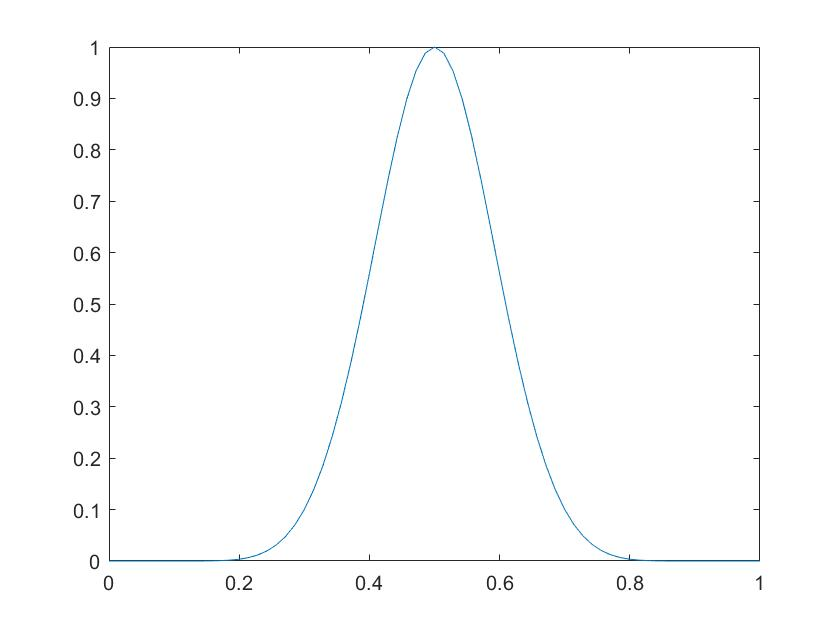
\includegraphics[scale=0.25]{Pert2.jpg}
		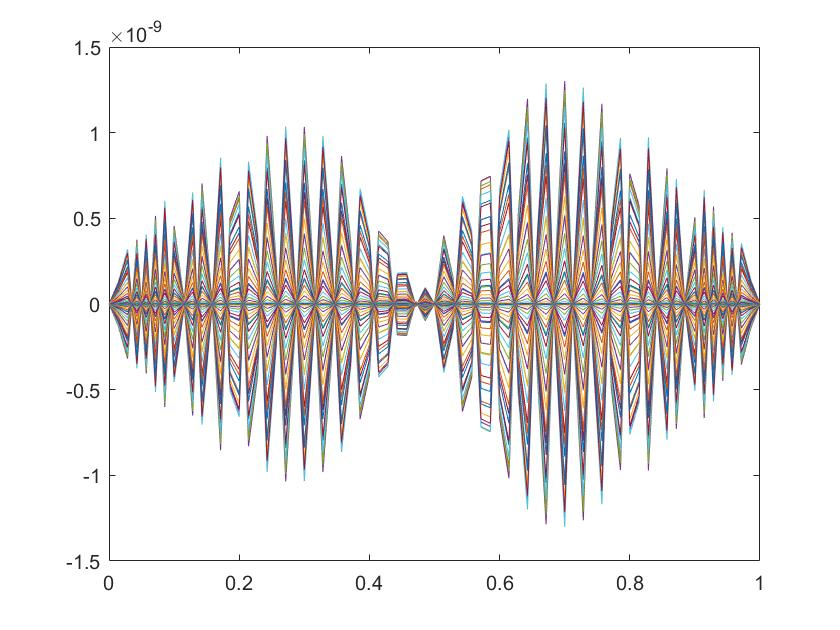
\includegraphics[scale=0.25]{ErrPert2.jpg}
		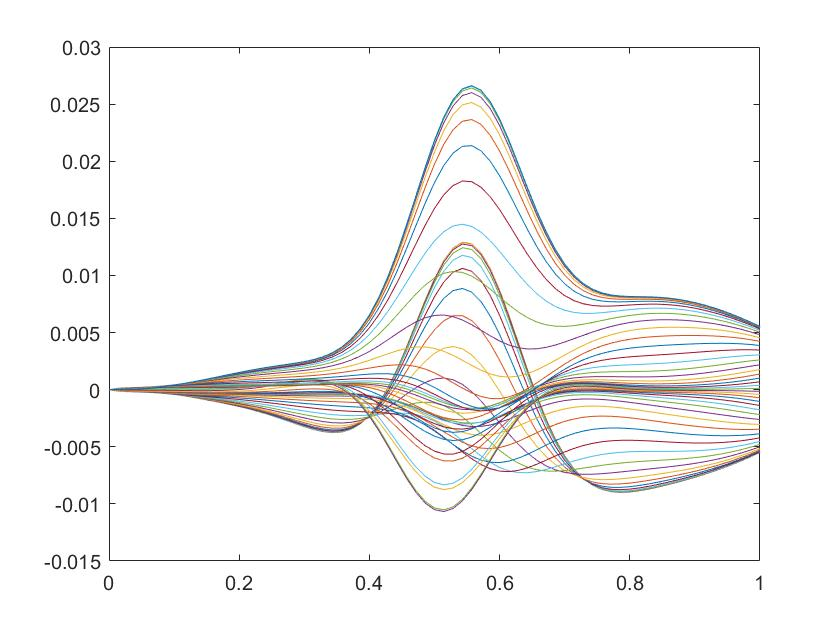
\includegraphics[scale=0.25]{ErrrhoPert2.jpg}
		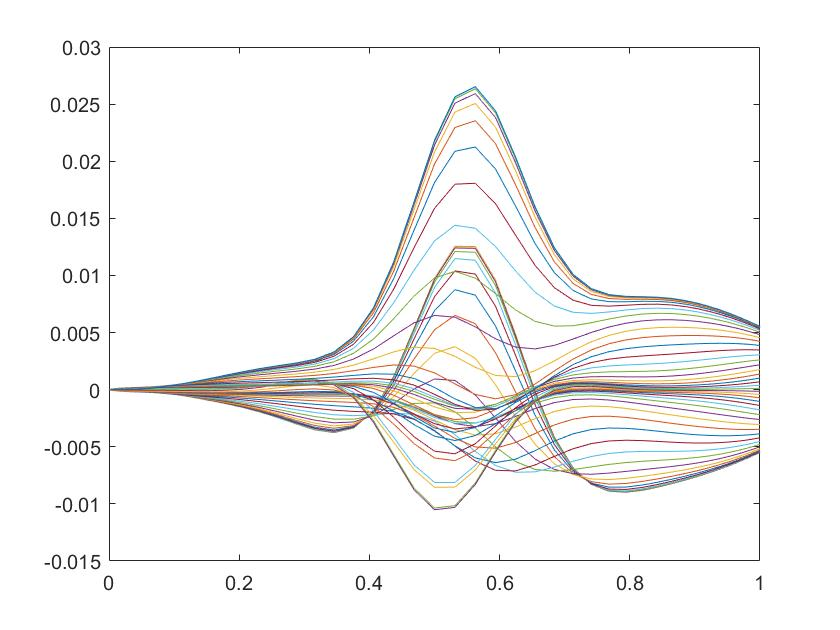
\includegraphics[scale=0.25]{ErrrhoPert2b.jpg}
		\caption{Interpolation Error in $w$ due to the perturbation and resulting error in $rho_{Opti}$ vs $rho_{Ex}$ (left equi, right Cheb). Note, $\rho$ did not converge! In L2Linf relative norm it is:$2.5362e-10$. }
		\label{Pert1}
	\end{figure}
    \begin{figure}[h]
		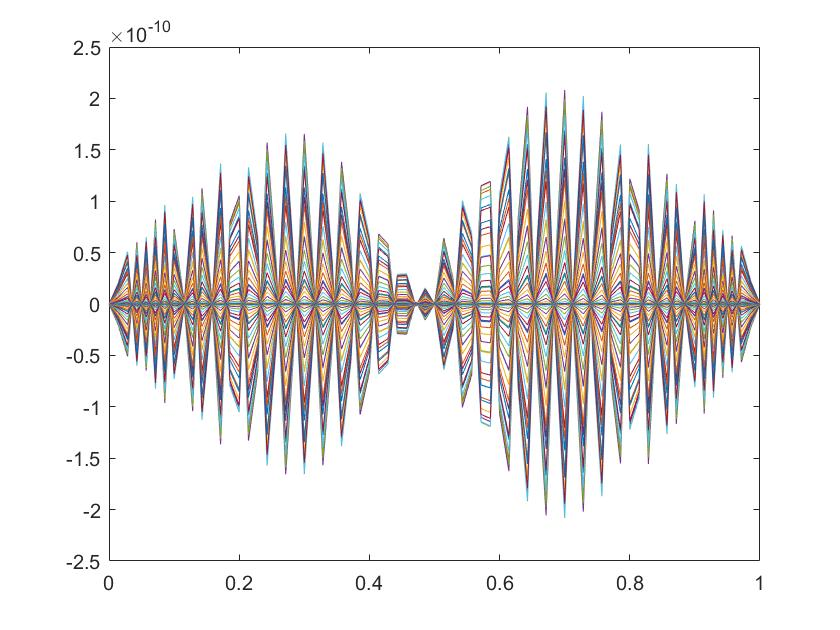
\includegraphics[scale=0.25]{ErrPert2a.jpg}
		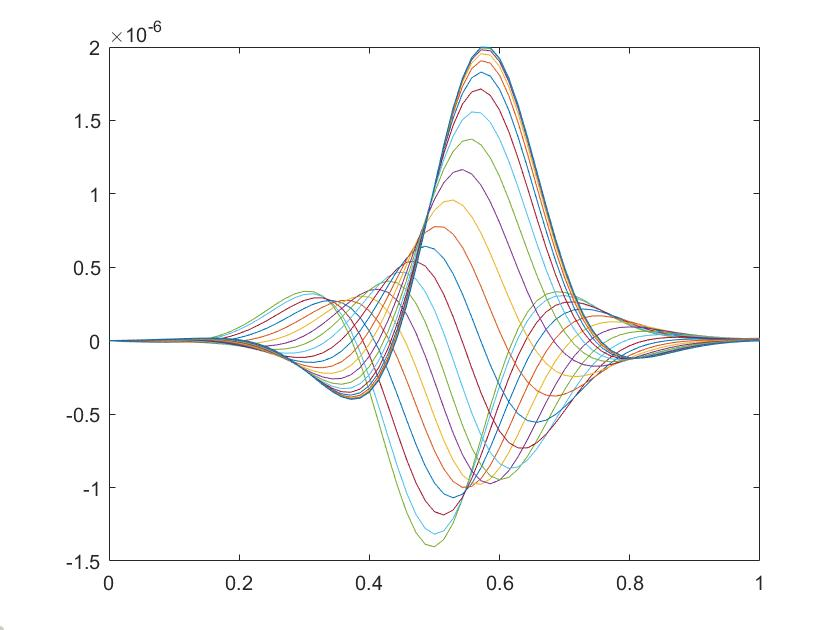
\includegraphics[scale=0.25]{ErrrhoPert2a.jpg}
		\caption{Interpolation Error in $w$ due to the perturbation and resulting error in $rho_{Opti}$ vs $rho_{Ex}$ (left equi, right Cheb). $\rho$ converged. In L2Linf relative norm it is:$1.4398e-10$. }
		\label{Pert2}
	\end{figure}
	
	When the scaling parameter in $\tilde g$ is $a = 0.5$ we have the following results. For $1\rho$ and $1p$ scaling, again this does not converge. See Figure \ref{Pert3}. Again, for $0.4\rho$, $0.4 p$ the problem converges, but the error in $\rho$ looks very different. See Figures \ref{Pert3} and \ref{Pert4}.
		\begin{figure}[h]
		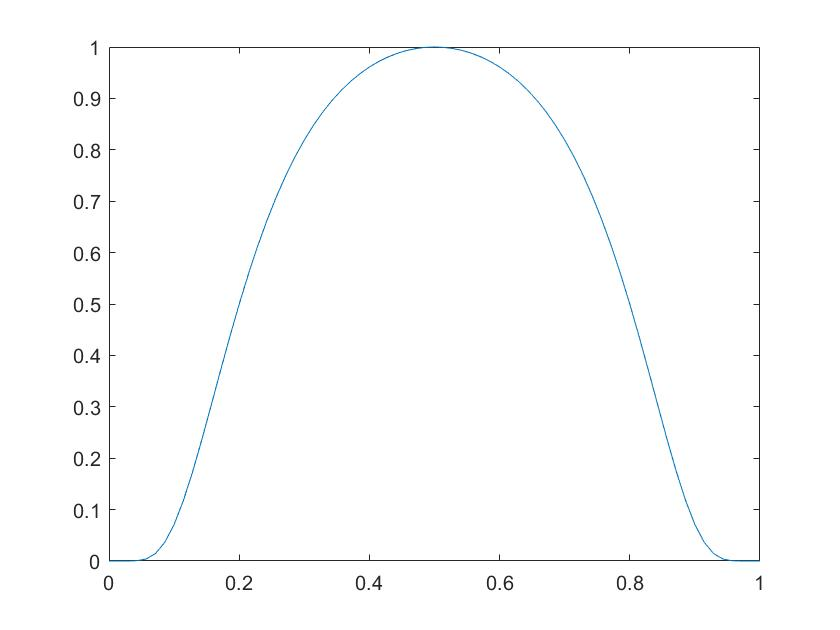
\includegraphics[scale=0.25]{Pert05.jpg}
		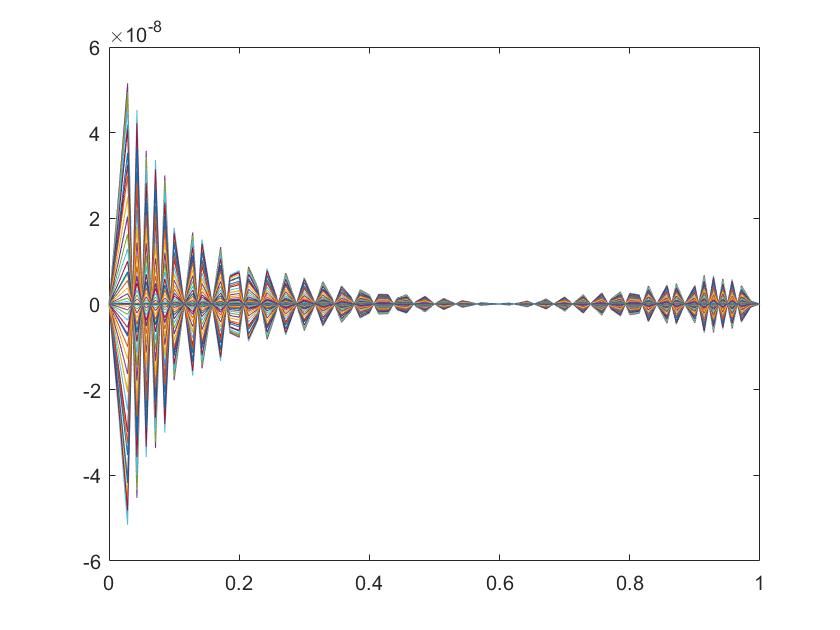
\includegraphics[scale=0.25]{ErrPert05.jpg}
		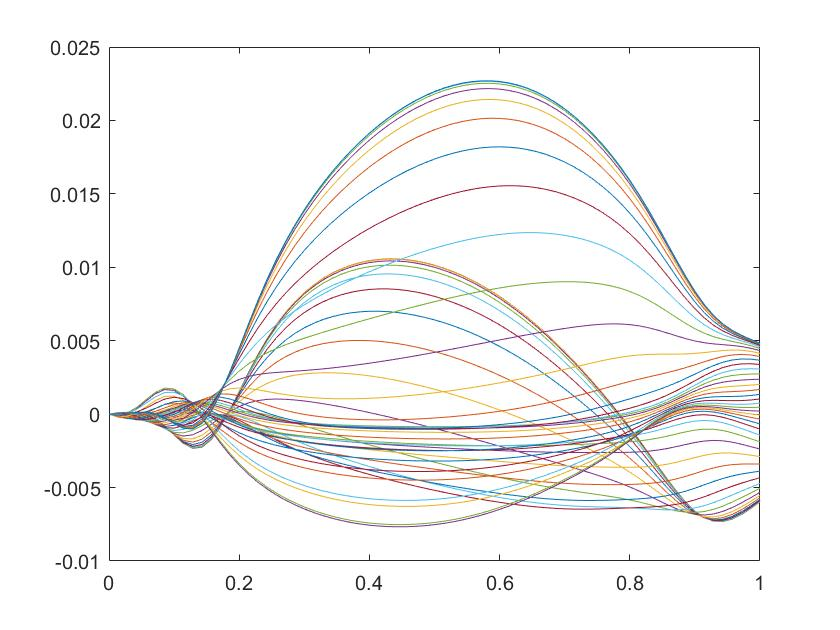
\includegraphics[scale=0.25]{ErrrhoPert05.jpg}
		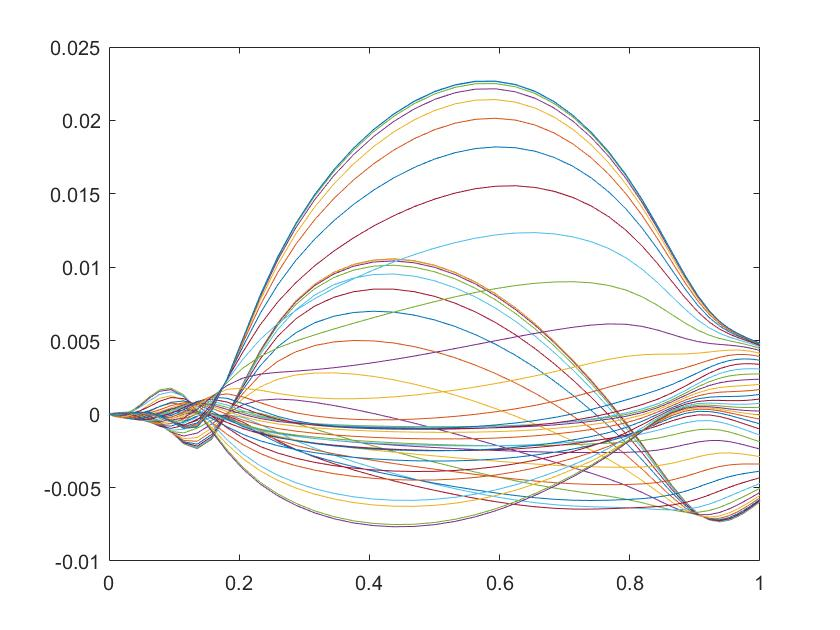
\includegraphics[scale=0.25]{ErrrhoPert05b.jpg}
		\caption{Interpolation Error in $w$ due to the perturbation and resulting error in $rho_{Opti}$ vs $rho_{Ex}$ (left equi, right Cheb). Note, $\rho$ did not converge! In L2Linf relative norm it is:$4.3039e-09$. }
		\label{Pert3}
	\end{figure}
		\begin{figure}[h]
		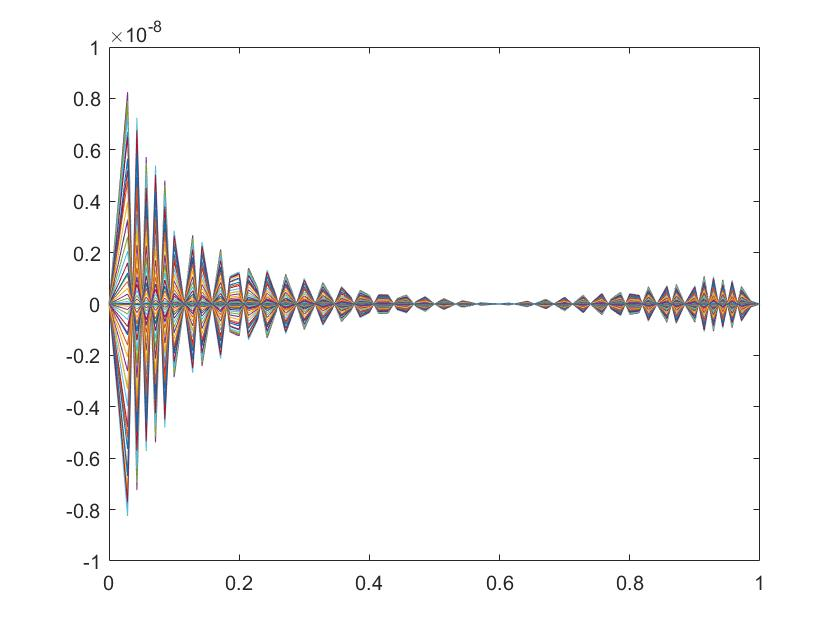
\includegraphics[scale=0.25]{ErrPert05a.jpg}
		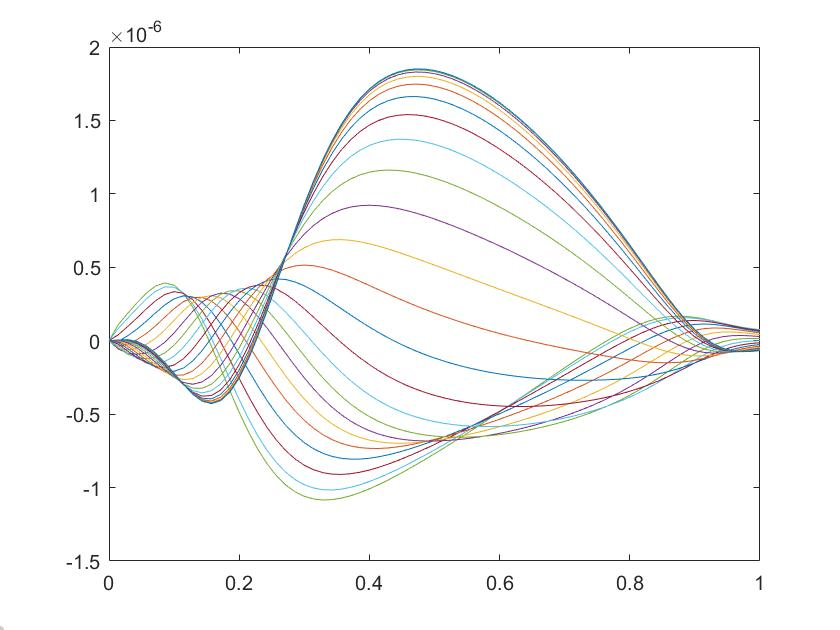
\includegraphics[scale=0.25]{ErrrhoPert05a.jpg}
		\caption{Interpolation Error in $w$ due to the perturbation and resulting error in $rho_{Opti}$ vs $rho_{Ex}$ (left equi, right Cheb). $\rho$ converged. In L2Linf relative norm it is:$4.3039e-09$. }
		\label{Pert4}
	\end{figure}
Conclusion: there doesn't seem to be a problem with time interpolation. The interpolation error for $w$ is within the norm. However, it does seem to correlate with the steepness of the perturbation function (?!).
The bigger $\rho$ and $p$ are, the 'weirder' are the errors in $\rho$ (Opti vs Exact).
\subsection{Checking how varying $\tilde g$ parameter $a$ changes $\rho$}
	In Figure \ref{gTest}, there are the three considered perturbations applied to $w$. In Figure \ref{gTest1}, the effect of these on $2\rho$ is displayed and in Figure \ref{gTest2} the effect on $0.5 \rho$. The location of the 'fold' does not seem to be correlated with the shape of $\tilde g(t)$.
	\begin{figure}[h]
		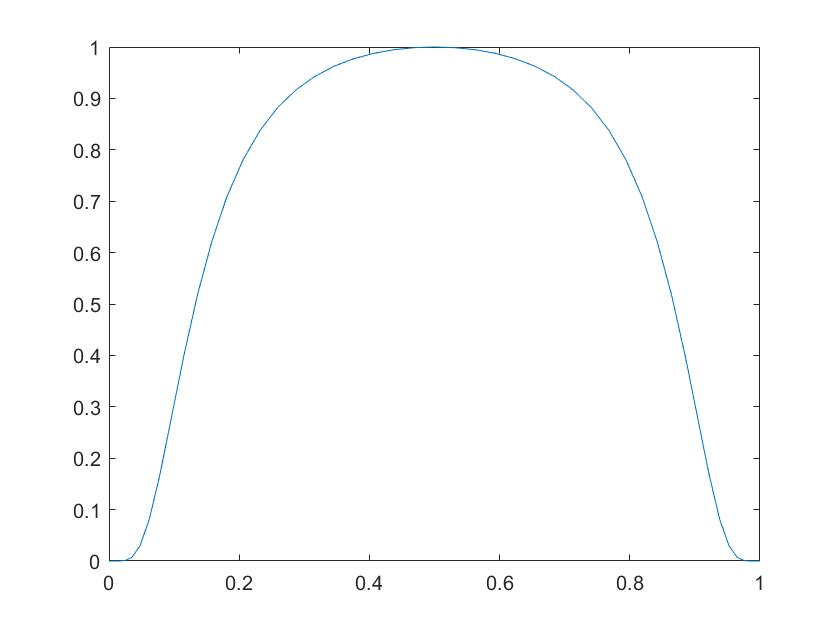
\includegraphics[scale=0.25]{Pert03new.jpg}
		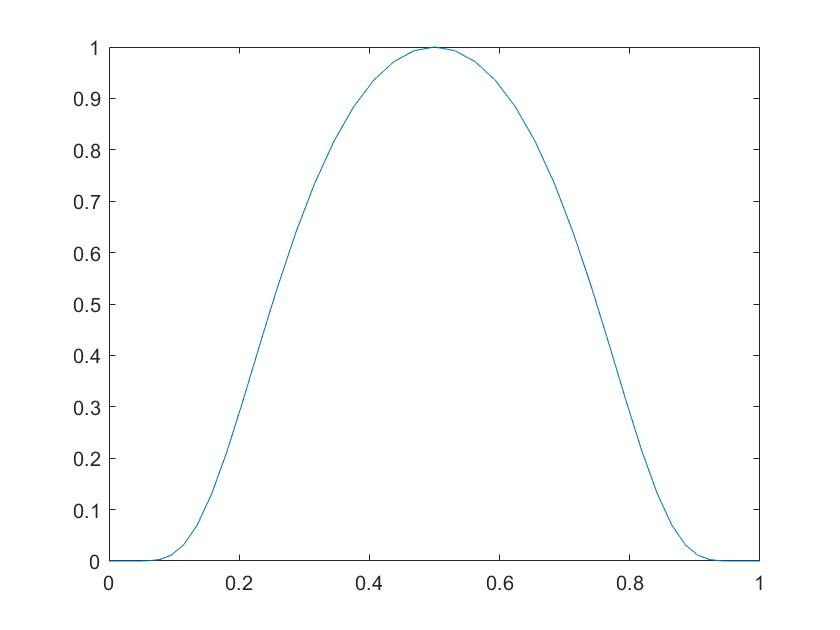
\includegraphics[scale=0.25]{Pert07new.jpg}
		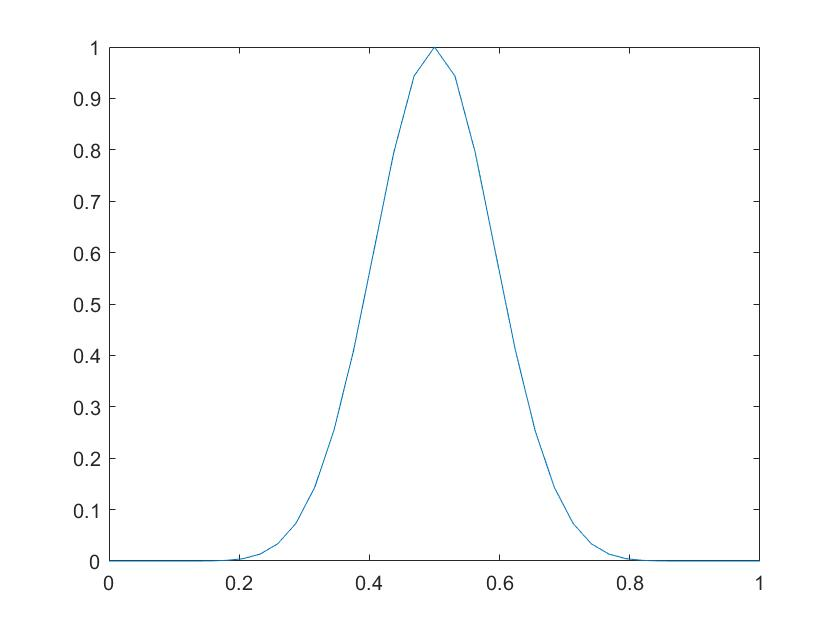
\includegraphics[scale=0.25]{Pert2new.jpg}
		\caption{ $\tilde g(t)$ with $a = 0.3$, $a=0.7$ and $a = 2$. }
		\label{gTest}
	\end{figure}
	\begin{figure}[h]
		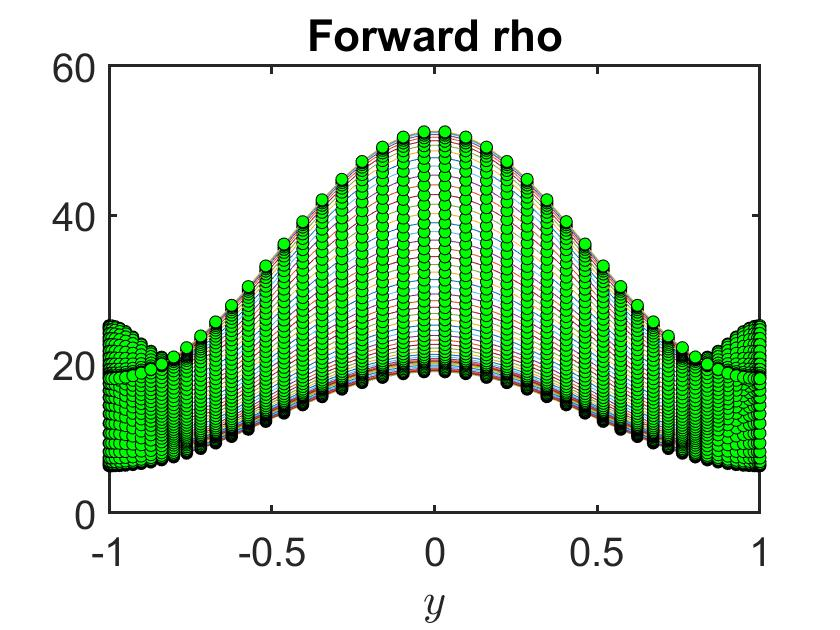
\includegraphics[scale=0.25]{rho203.jpg}
		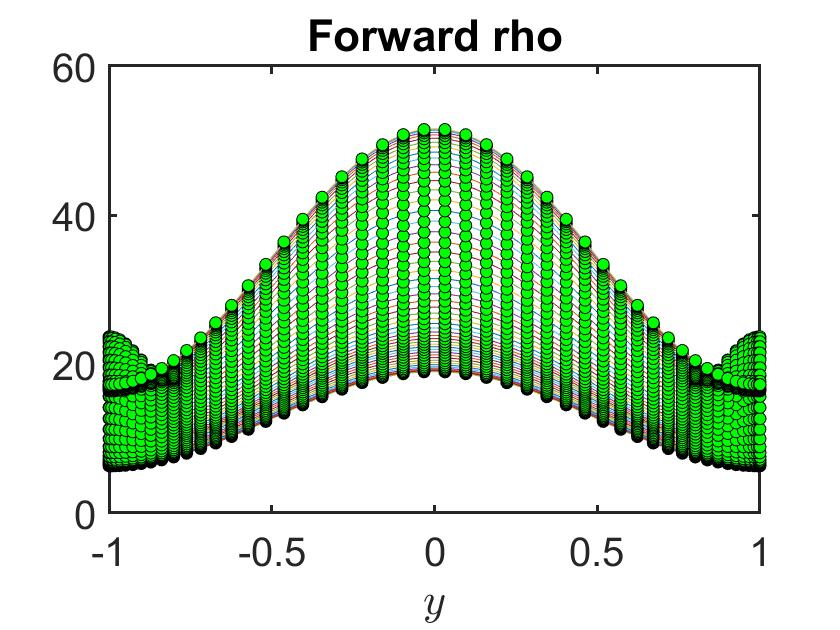
\includegraphics[scale=0.25]{rho207.jpg}
		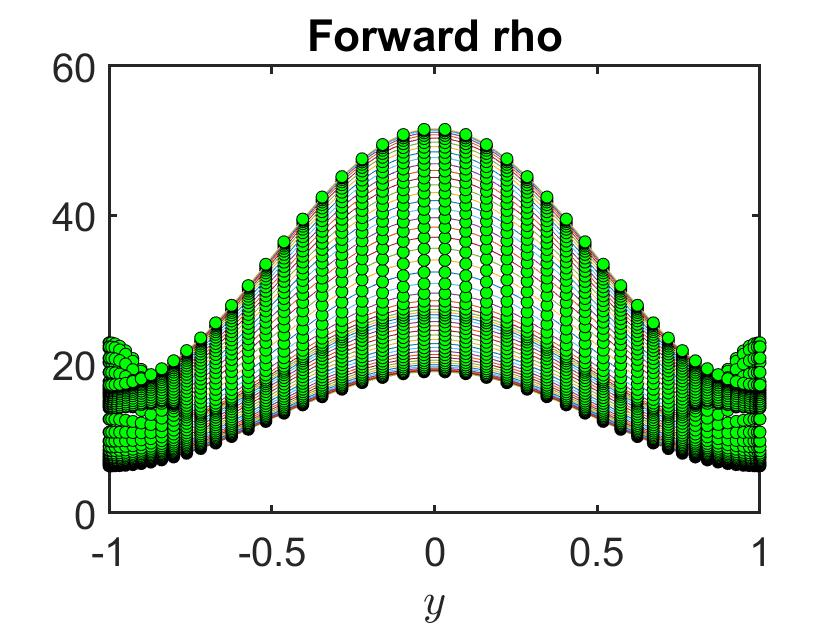
\includegraphics[scale=0.25]{rho22.jpg}
		\caption{$2\rho$ forward solution for $w$ perturbed by $0.1 \tilde g(t)$, with $a = 0.3$, $a=0.7$ and $a = 2$. }
		\label{gTest1}
	\end{figure}
	
	\begin{figure}[h]
		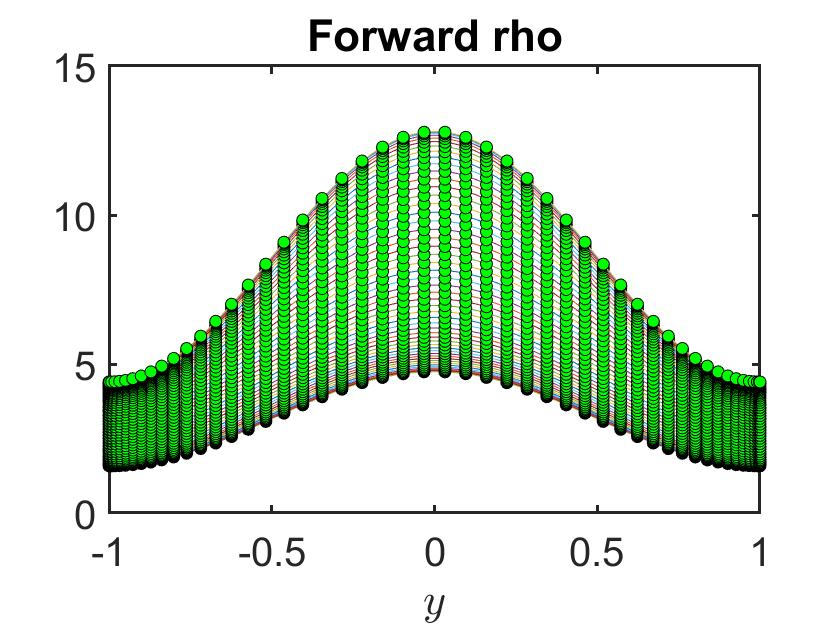
\includegraphics[scale=0.25]{rho0503.jpg}
		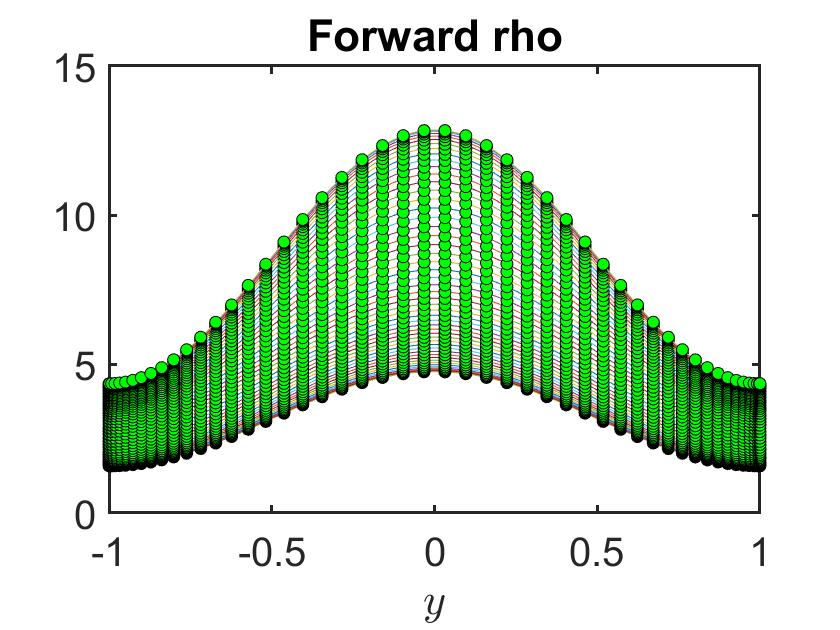
\includegraphics[scale=0.25]{rho0507.jpg}
		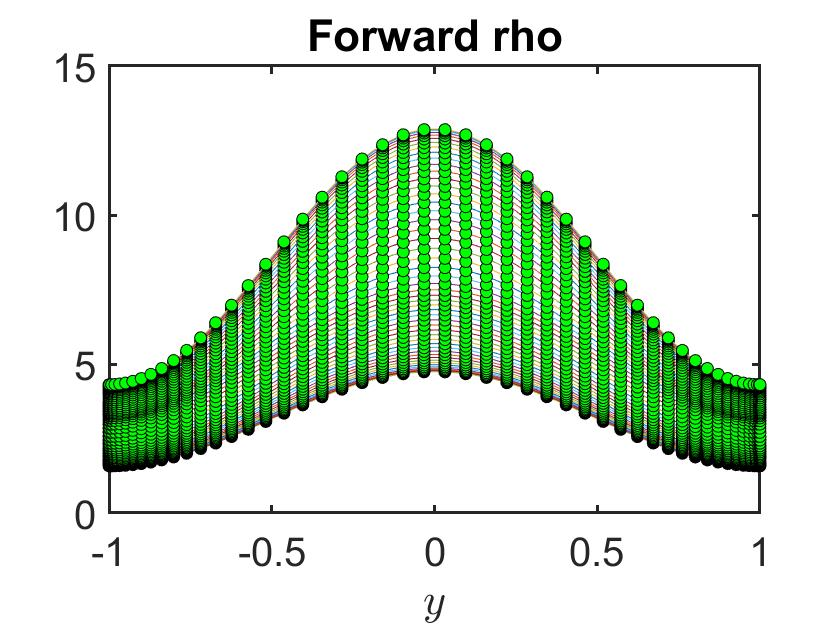
\includegraphics[scale=0.25]{rho052.jpg}
		\caption{$0.5\rho$ forward solution for $w$ perturbed by $0.1 \tilde g(t)$, with $a = 0.3$, $a=0.7$ and $a = 2$. }
		\label{gTest2}
	\end{figure}
	
	
\subsection{Investigating $\rho = e^h$}	
	Rewriting the forward equation in terms of $\rho = e^h$:
	\begin{align*}
	\partial_t \rho &= \Delta \rho - \nabla \cdot (w \rho) + f\\
	\partial_t h &= \Delta h + \nabla h \cdot \nabla h - \nabla \cdot w + \nabla h \cdot w + fe^{-h}.
	\end{align*}
	
	Checked code on Diffusion case first. Works. (FW solution = exact solution). Forward Case in AD works too.

\section{Quick investigation on Interacting problems}
First tried the same exact solutions as the Neumann flow control ones, but $ \beta$ fully on $p$, and $\rho$, $w$ independent of it. However, the PDE is the Flow control PDE without Force term and with included particle interaction term.
If we scale $\rho$ and $p$ such that $w$ is order 1, this works well.
Tested for $\gamma = 1$ and $\gamma = -1$. Some problems have been tested with Picard, some with PixPt. Different values of $\beta$ have been investigated.
All of these problems converge, however it is noticeable that the cost functionals are very close together. The optimal solution does better, but only marginally so. Furthermore, it seems that the Forward solution doesn't change so much with $\gamma$, see Figure \ref{gamma1}. For $1\rho$ the impact on gamma is stronger. Already for $0.4\rho$ and $0.2 p$ the problem diverges for $\beta =10^{-3}$ (but converges for $\beta = 10^{-1}$) This is equivalent to $w$ of order 2.\\
    \begin{figure}[h]
		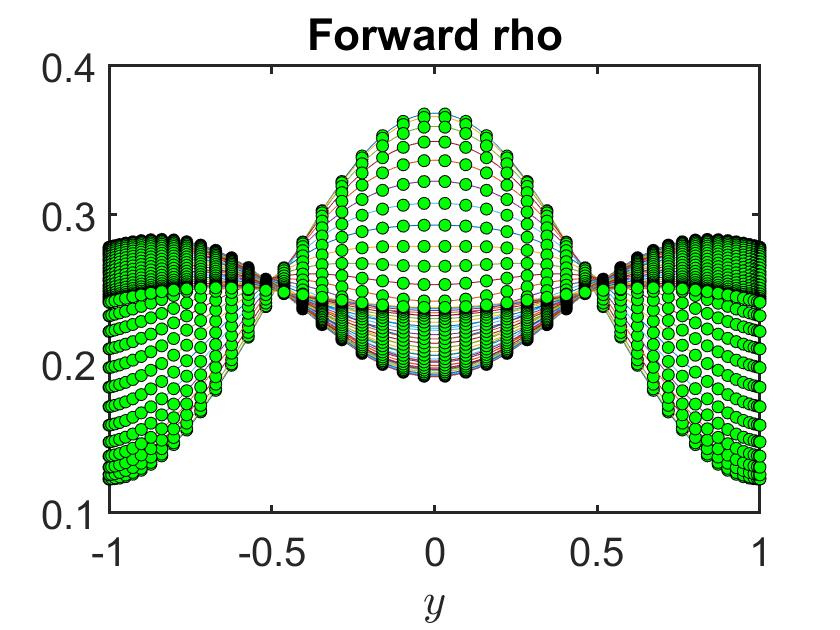
\includegraphics[scale=0.25]{gamma1.jpg}
		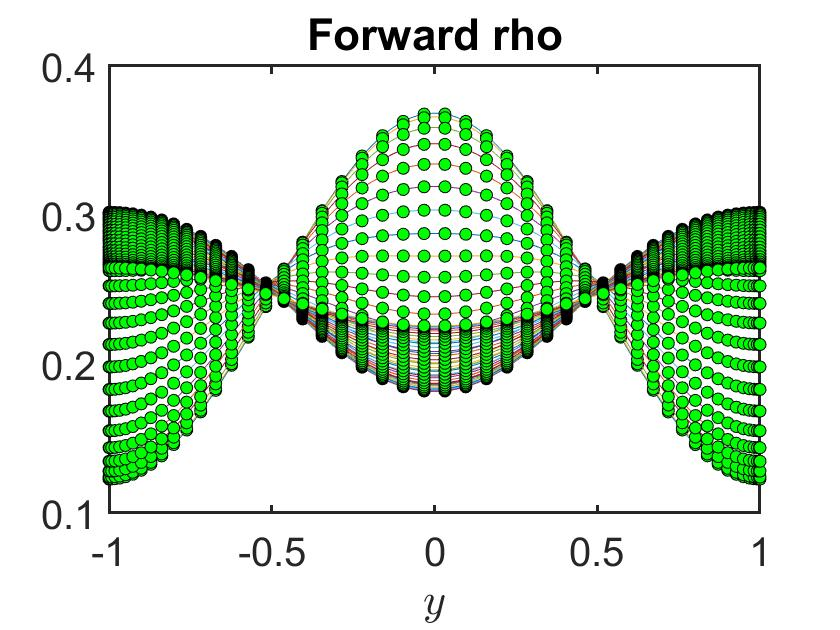
\includegraphics[scale=0.25]{gamma0.jpg}
		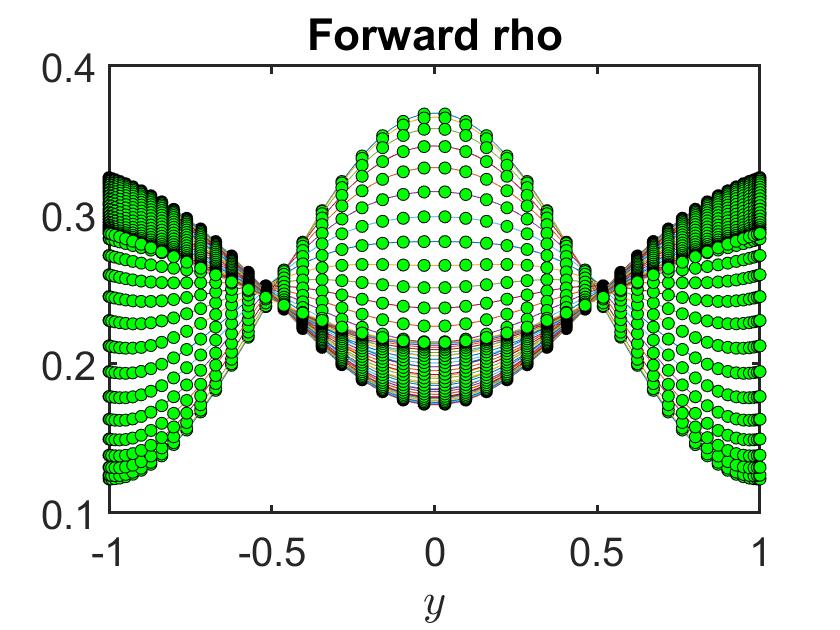
\includegraphics[scale=0.25]{gamma11.jpg}
		\caption{$1/8.1441\rho$ forward solution with $\gamma = -1,0,1$ }
		\label{gamma1}
	\end{figure}
	\begin{figure}[h]
	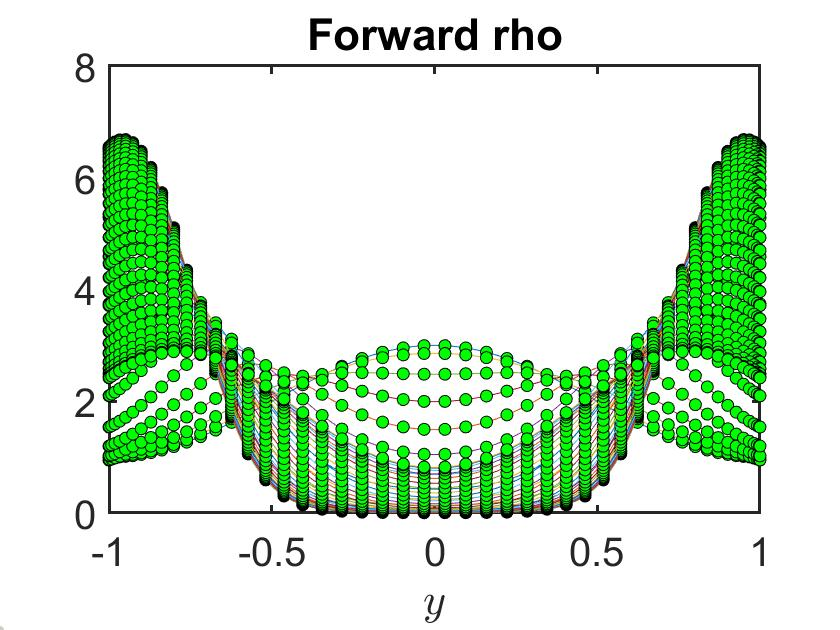
\includegraphics[scale=0.25]{gamman1a.jpg}
	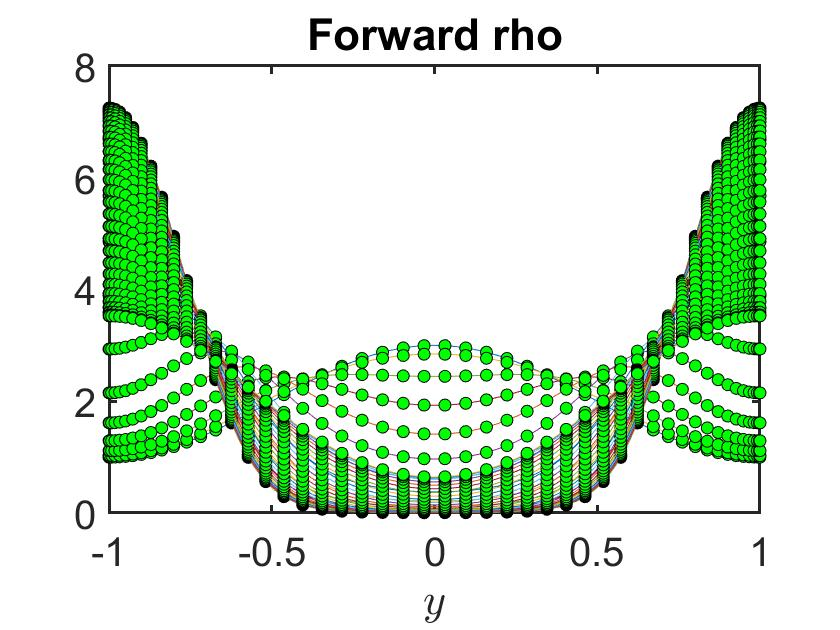
\includegraphics[scale=0.25]{gamma0a.jpg}
	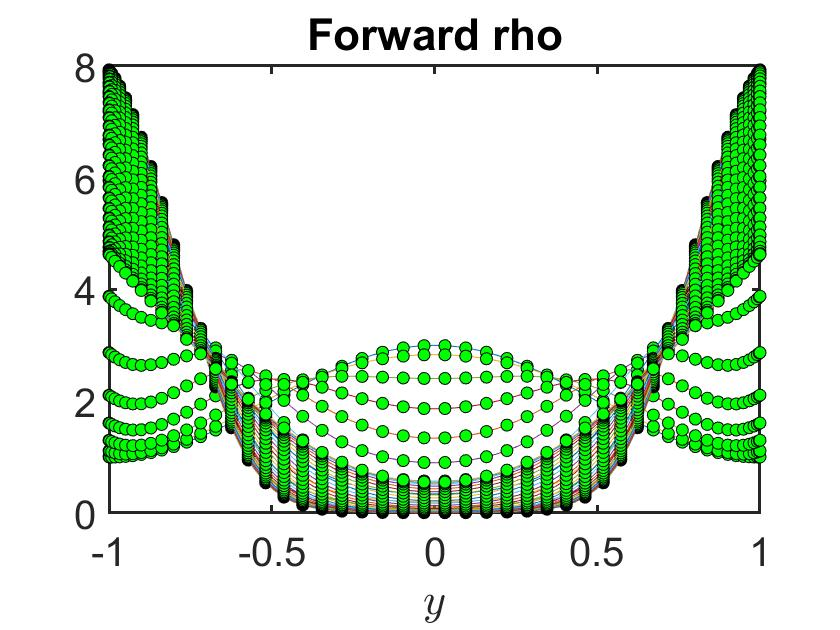
\includegraphics[scale=0.25]{gamma1a.jpg}
	\caption{$1\rho$ forward solution with $\gamma = -1,0,1$ }
	\label{gamma2}
    \end{figure}

The next idea was that $\hat \rho$ should be independent of $\beta$ as well. Chose
\begin{align*}
\hat \rho = \cos( \pi y + \pi/2) +2.
\end{align*}
This is a shift in the shape but not a change in mass. 
Using the scaling that $w$ is of order $1$, this converges for $\beta = 10^{-1}$, but not for $\beta = 10^{-3}$. Changed $\hat \rho$ to $\hat \rho = \cos( \pi y + \pi/4) +2$ in case it is easier but it didn't improve the situation.\\
Need to think of a better problem but also looks like a similar issue to the one with large $w$.
	
	
\end{document}